\section{Observations}

\begin{enumerate}
    \item \textbf{RS Flip-flop using NOR gates}\\
    Refer to Fig. \ref{1}.
    \begin{table}[H]
        \centering
        \begin{tabular}{|c|c|c|c|c|}\hline
            $R$ & $S$ & $Q$ & $Q'$ & Remark \\ \hline
            0 & 1 & 1 & 0 & \verb|SET| \\ 
            0 & 0 & 1 & 0 & \verb|HOLD| \\ 
            1 & 0 & 0 & 1 & \verb|RESET| \\ 
            0 & 0 & 0 & 1 & \verb|HOLD| \\ 
            1 & 1 & 0 & 0 & Invalid \\ \hline
        \end{tabular}
        \caption{Observed characteristic Table for an RS Flip-Flop}
    \end{table}

    \item \textbf{RS Flip-flop using NAND gates}\\
    
    \begin{figure}[H]
        \centering
        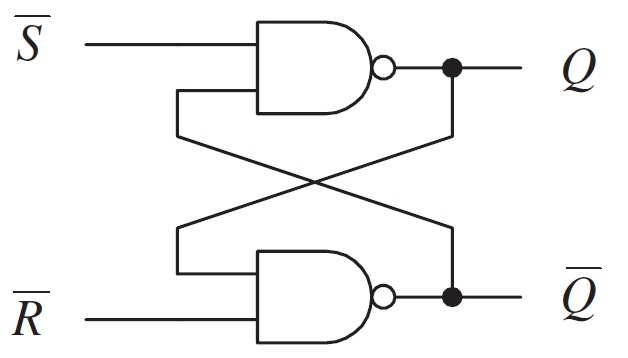
\includegraphics[width=0.50\columnwidth]{images/rsnand.jpg}
        \caption{Circuit diagram of an RS flip-flop using NAND gates. $Q$ and $Q'$ are instead configured at S' and R' respectively, unlike Fig \ref{1}.}
    \end{figure}

    \begin{table}[H]
        \centering
        \begin{tabular}{|c|c|c|c|c|}\hline
            $S'$ & $R'$ & $Q$ & $Q'$ & Remark \\ \hline
            0 & 1 & 1 & 0 & \verb|SET| \\ 
            1 & 1 & 1 & 0 & \verb|HOLD| \\ 
            1 & 0 & 0 & 1 & \verb|RESET| \\ 
            1 & 1 & 0 & 1 & \verb|HOLD| \\ 
            0 & 0 & 0 & 0 & Invalid \\ \hline
        \end{tabular}
        \caption{Observed characteristic Table for an RS Flip-Flop using NAND gates.}
    \end{table}

    \noindent Notice how the indeterminate state is defined when $S=R=0$ and the Hold state is when $S=R=1$, due to the fundamental difference between NAND and NOR properties.\\

    \item \textbf{Gated RS Flip-flop}\\
    Refer to Fig. \ref{2}.
    \begin{table}[H]
        \centering
        \begin{tabular}{|c|c|c|c|c|}\hline
            $Q_N$ & $R$ & $S$ & $Q_{N+1}$ & Remark \\ \hline
            0 & 1 & 0 & 0 & \verb|RESET| \\ 
            0 & 0 & 0 & 0 & \verb|HOLD|\\ 
            0 & 0 & 1 & 1 & \verb|SET|\\ 
            1 & 0 & 0 & 1 & \verb|HOLD| \\ 
            1 & 0 & 1 & 1 & \verb|SET| \\ 
            1 & 1 & 0 & 0 & \verb|RESET|\\ 
            0 & 1 & 1 & 0 & Indeterminate\\ 
            1 & 1 & 1 & 0 & Indeterminate\\\hline
        \end{tabular}
        \caption{Observed characteristic Table for a gated RS Flip-Flop}
    \end{table}

    \item \textbf{D Flip-flop}\\
    Refer to Fig. \ref{3}.
    \begin{table}[H]
        \centering
        \begin{tabular}{|c|c|c|c|c|}\hline
            $Q_N$ & $D$ & $Q_{N+1}$ \\ \hline
            0 & 1 & 1 \\ 
            1 & 0 & 0 \\ 
            0 & 1 & 1 \\ 
            1 & 1 & 1 \\ \hline
        \end{tabular}
        \caption{Observed characteristic Table for a gated RS Flip-Flop, with Clk $=1$}
    \end{table}

    \item \textbf{JK Flip-flop}\\
    Refer to Fig. \ref{4}.
    \begin{table}[H]
        \centering
        \begin{tabular}{|c|c|c|c|c|}\hline
            $Q_N$ & $J$ & $K$ & $Q_{N+1}$ & Remark \\ \hline
            0 & 0 & 0 & 0 & \verb|HOLD| \\ 
            0 & 0 & 1 & 0 & \\ 
            0 & 1 & 0 & 1 & \\ 
            1 & 0 & 1 & 0 & \\ 
            1 & 1 & 0 & 1 & \\
            1 & 0 & 0 & 1 & \verb|HOLD|\\ 
            1 & 1 & 1 & 0 & \verb|TOGGLE| \\ 
            0 & 1 & 1 & 1 & \verb|TOGGLE| \\ \hline
        \end{tabular}
        \caption{Observed characteristic Table for a JK Flip-Flop}
    \end{table}

    \item \textbf{Master-Slave JK Flip-flop}\\
    Refer to Fig. \ref{5}.
    \begin{table}[H]
        \centering
        \begin{tabular}{|c|c|c|c|c|c|c|}\hline
            CP &$J$ & $K$ & $Q_m$ & $ Q'_m$ & $Q_n$ & $ Q'_n$ \\ \hline
            $0 \rightarrow 1$ & 0 & 1 & 0 & 1 & \multicolumn{2}{c|}{Hold} \\ \hline
            $1 \rightarrow 0$ & 0 & 1 & \multicolumn{2}{c|}{Hold} & 0 & 1 \\ \hline
            $0 \rightarrow 1$ & 1 & 0 & 1 & 0 & \multicolumn{2}{c|}{Hold}\\ \hline
            $1 \rightarrow 0$ & 1 & 0 & \multicolumn{2}{c|}{Hold} & 1 & 0\\ \hline
            $0 \rightarrow 1$ & 0 & 0 & \multicolumn{2}{c|}{Hold} & \multicolumn{2}{c|}{Hold} \\ \hline
            $1 \rightarrow 0$ & 0 & 0 & \multicolumn{2}{c|}{Hold} & \multicolumn{2}{c|}{Hold} \\ \hline
            $0 \rightarrow 1$ & 1 & 1 & \multicolumn{2}{c|}{Toggle} & \multicolumn{2}{c|}{Hold} \\\hline
            $1 \rightarrow 0$ & 1 & 1 & \multicolumn{2}{c|}{Hold} & \multicolumn{2}{c|}{Toggle} \\ \hline
        \end{tabular}
        \caption{Observed characteristic Table for a Master-Slave JK Flip-Flop}
    \end{table}

    \item \textbf{JK Flip-flop}\\
    Refer to Fig. \ref{5}, where J \& K are set to 1.
    \begin{table}[H]
        \centering
        \begin{tabular}{|c|c|c|c|}\hline
            $Q_N$ & $T$ & $Q_{N+1}$ & Remark\\ \hline
            0 & 0 & 0 & \verb|HOLD| \\ 
            0 & 1 & 1 & \verb|TOGGLE| \\ 
            1 & 0 & 1 & \verb|HOLD| \\ 
            1 & 1 & 0 & \verb|TOGGLE|\\ \hline
        \end{tabular}
        \caption{Observed characteristic Table for a T Flip-Flop}
    \end{table}

\end{enumerate}